\chapter{IMPLEMENTASI}
Pada bab ini akan dipaparkan implementasi dari sistem yang dibangun. Bahasa pemrograman yang digunakan adalah HTML, CSS, Javascript, dan PHP yang dikemas dalam framework Laravel.

\section{Lingkungan Implementasi}
\tab Lingkungan implementasi dalam pembuatan sistem pada kerja praktik kali ini meliputi perangkat keras dan perangkat lunak yang digunakan untuk mengimplementasikan sistem yang telah dirancang adalah sebagai berikut:
\begin{enumerate}
	\item Perangkat Keras
	\begin{itemize}
	\item \textit{Processor} Intel® Core™ i7-5500U CPU @ 2.40GHz
	\item Memori 4 GB
	\end{itemize}
	\item Perangkat Lunak
	\begin{itemize}
	\item Sistem Operasi Ubuntu 16.04 LTS 64 bit.
	\item \textit{Text editor} Visual Studio Code
	\item Bahasa pemrograman PHP.
	\end{itemize}
\end{enumerate}

\section{Tampilan Fitur Aplikasi TPORT}
Berikut adalah tampilan aplikasi TPORT.

\subsection{Tampilan Halaman \textit{Request} TPORT}
Tampilan halaman \textit{request} TPORT menggunakan bahasa pemrograman HTML, CSS, Javascript dan PHP untuk tampilan sistem. Penampilan data pada halaman ini bersifat dinamis. Semua fitur pada aplikasi TPORT didaftar secara rinci dan dikemas dalam tampilan statis. Kemudian ketika salah satu fitur dipilih oleh user, maka akan diarahkan pada halaman sesuai fitur yang dipilih. Gambar \ref{figure:requestTPORT} dan \ref{figure:detailRequestTPORT} adalah tampilan halaman dan \ref{lst:request} adalah potongan kode dari halaman \textit{request} TPORT.

\begin{figure}[h!]
	\centerline
	{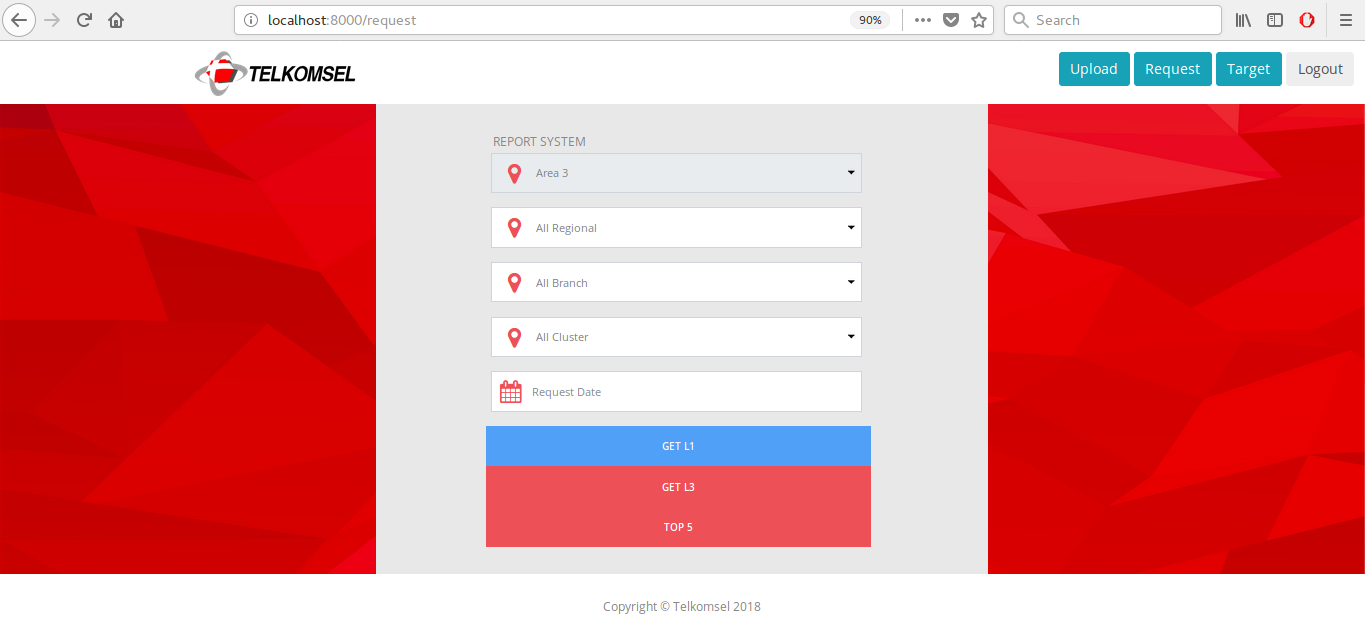
\includegraphics[width=10cm,height=5cm]{bab5/tampilanRequest.png}}
	\caption{Halaman \textit{Request} TPORT}
	\label{figure:requestTPORT}
\end{figure}

\begin{figure}[h!]
	\centerline
	{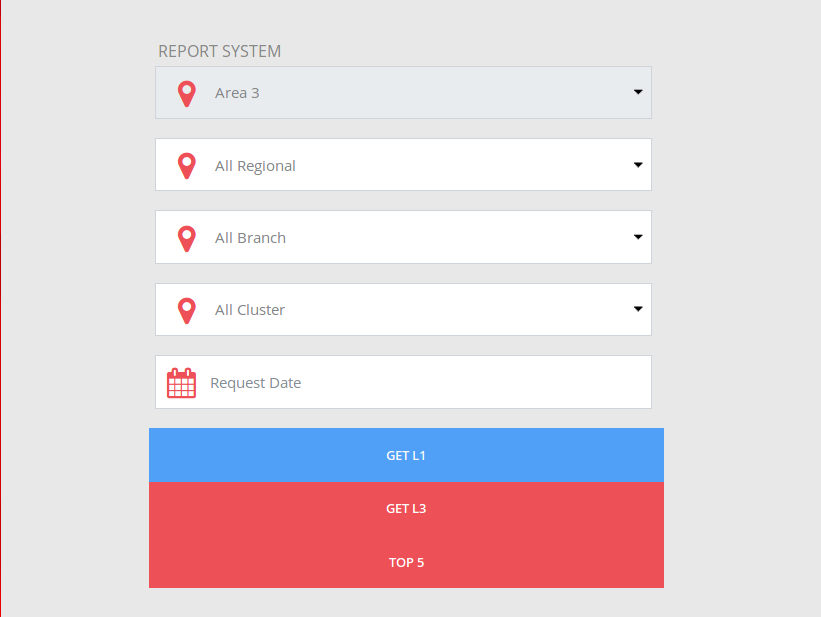
\includegraphics[width=10.5cm,height=7.5cm]{bab5/detailTampilanRequest.png}}
	\caption{Detail \textit{Form} pada Halaman \textit{Request} TPORT}
	\label{figure:detailRequestTPORT}
\end{figure}

\lstinputlisting[language=PHP, firstline=1, lastline=21, firstnumber=1, caption=Potongan Kode Tampilan Halaman \textit{Request} TPORT, label={lst:request}]{bab5/src/halamanReport.php}

\subsection{Tampilan Halaman \textit{Upload} TPORT}
Pada halaman menambahkan \textit{upload} TPORT bahasa yang digunakan adalah HTML, CSS, PHP dan Javascript. Sebuah \textit{form} akan ditampilkan dan kemudian pengguna akan mengisikan data-data sesuai spesifikasi file yang diupload. File yang diupload berupa file .csv (\textit{Comma Separated Values}). \textit{Form} tersebut akan menampung data-data yang diperlukan, kemudian akan disimpan ke dalam basis data sistem. Gambar \ref{figure:uploadTPORT} dan \ref{figure:detailUploadTPORT} adalah tampilan halaman \textit{upload} dan \ref{lst:uploadTPORT} adalah potongan kode halaman \textit{upload} TPORT.

\begin{figure}[h!]
\centerline
{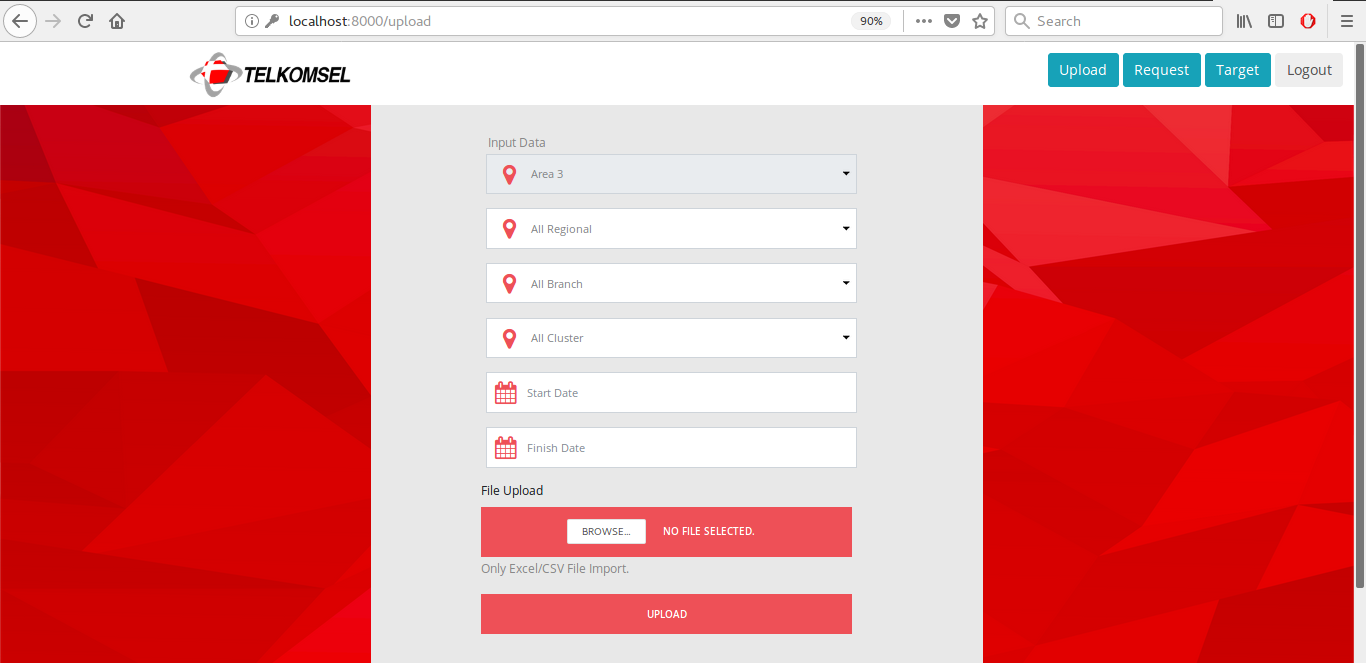
\includegraphics[width=10cm,height=5cm]{bab5/tampilanUpload.png}}
\caption{Halaman \textit{Upload} TPORT}
\label{figure:uploadTPORT}
\end{figure}

\begin{figure}[h!]
	\centerline
	{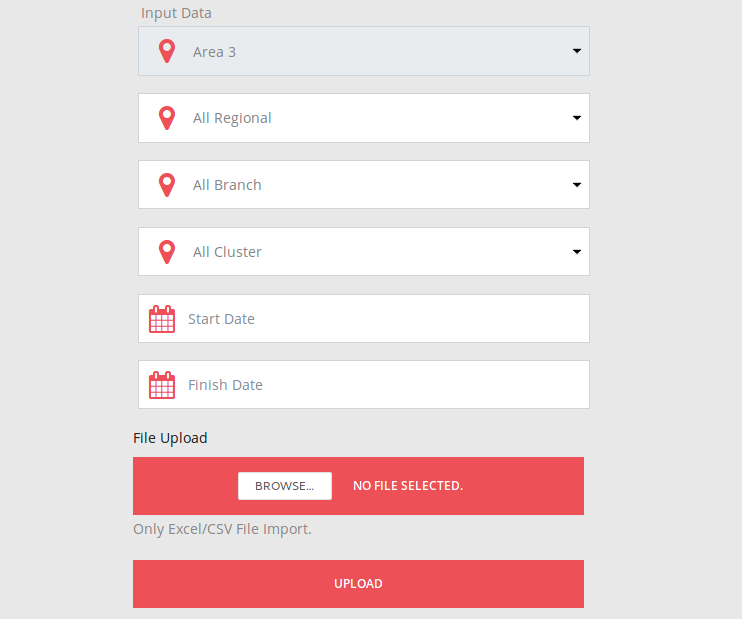
\includegraphics[width=10.5cm,height=7.5cm]{bab5/detailTampilanUpload.png}}
	\caption{Detail \textit{Form} pada Halaman \textit{Upload} TPORT}
	\label{figure:detailUploadTPORT}
\end{figure}


\lstinputlisting[language=PHP, firstline=1, lastline=59, firstnumber=1, caption=Potongan Kode Tampilan \textit{Upload} TPORT, label={lst:uploadTPORT}]{bab5/src/halamanUpload.php}

\subsection{Tampilan Halaman Target TPORT}
Pada halaman target TPORT bahasa yang digunakan adalah HTML, CSS, PHP dan Javascript. Sebuah \textit{form} akan ditampilkan kemudian pengguna mengisikan nilai \textit{revenue} sesuai target yang ingin diraih untuk tiap kluster. \textit{Form} tersebut akan menampung data-data yang diperlukan, kemudian akan disimpan ke dalam basis data sistem. Gambar \ref{figure:targetTPORT} dan \ref{figure:detailTargetTPORT} adalah tampilan halaman dan \ref{lst:targetTPORT} adalah potongan kode dari halaman target.

\lstinputlisting[language=PHP, firstline=1, lastline=43, firstnumber=1, caption=Potongan Kode Tampilan Target TPORT, label={lst:targetTPORT}]{bab5/src/halamanTarget.php}

\begin{figure}[h!]
	\centerline
	{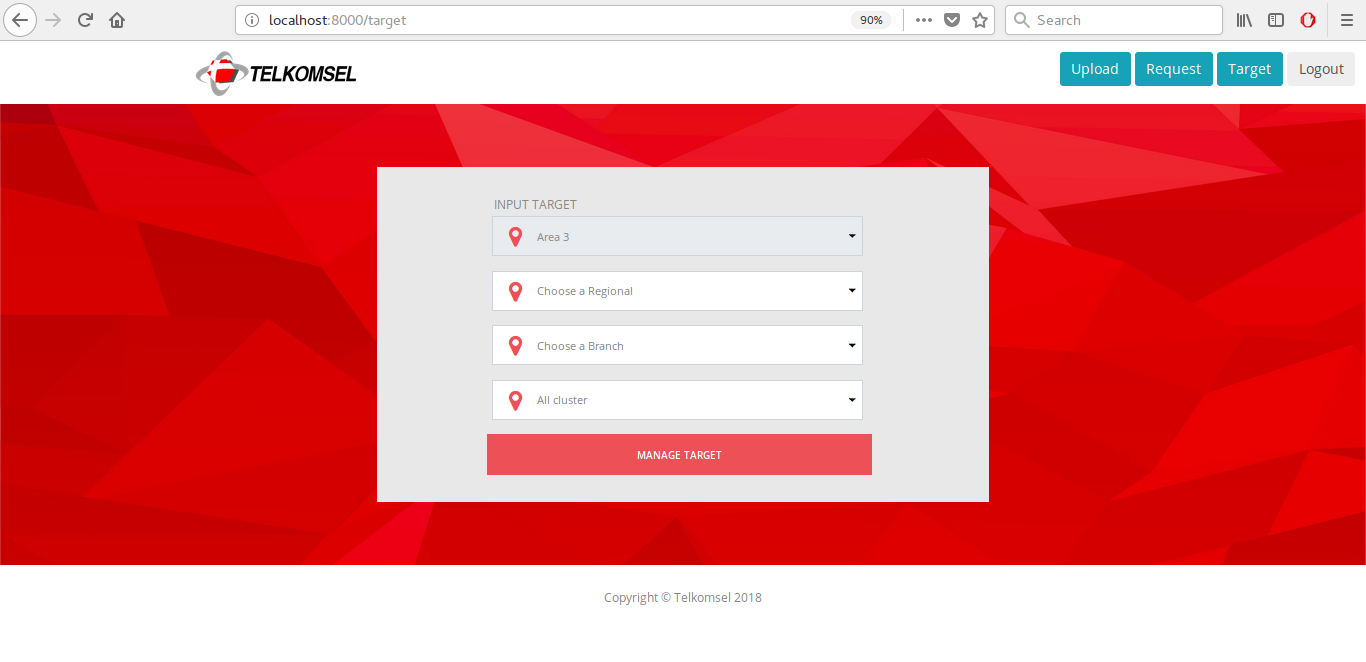
\includegraphics[width=10cm,height=5cm]{bab5/tampilanTarget.png}}
	\caption{Halaman Target TPORT}
	\label{figure:targetTPORT}
\end{figure}

\begin{figure}[h!]
	\centerline
	{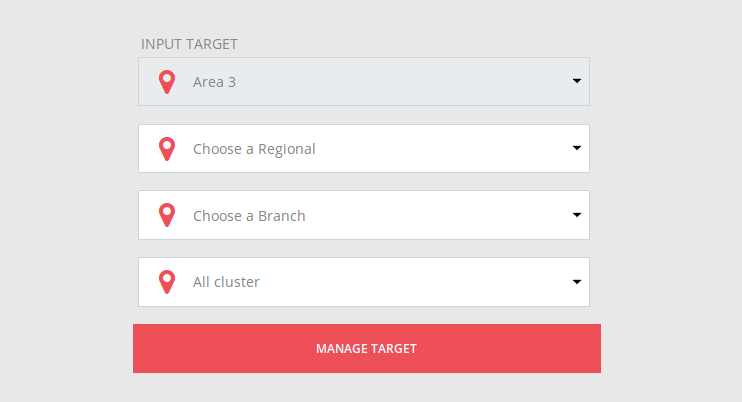
\includegraphics[width=10.5cm,height=6cm]{bab5/detailTampilanTarget.png}}
	\caption{Detail pada Halaman Target TPORT}
	\label{figure:detailTargetTPORT}
\end{figure}

\subsection{Halaman Pencapaian \textit{Revenue}}
Pada halaman pencapaian \textit{revenue} bahasa pemrograman yang digunakan adalah HTML, CSS dan PHP. Pada halaman ini, pengguna dapat melihat detail pencapaian \textit{revenue} berdasarkan wilayah, tanggal, dan kategori yang dipilih. Halaman ini akan menampilkan detail informasi sesuai pilihan pengguna tadi. Gambar \ref{figure:pencapaianTPORT} dan \ref{figure:detailPencapaianTPORT} adalah tampilan halaman dan \ref{lst:pencapaianTPORT} adalah potongan kode dari halaman detail pencapaian \textit{revenue}.

\begin{figure}[h!]
	\centerline
	{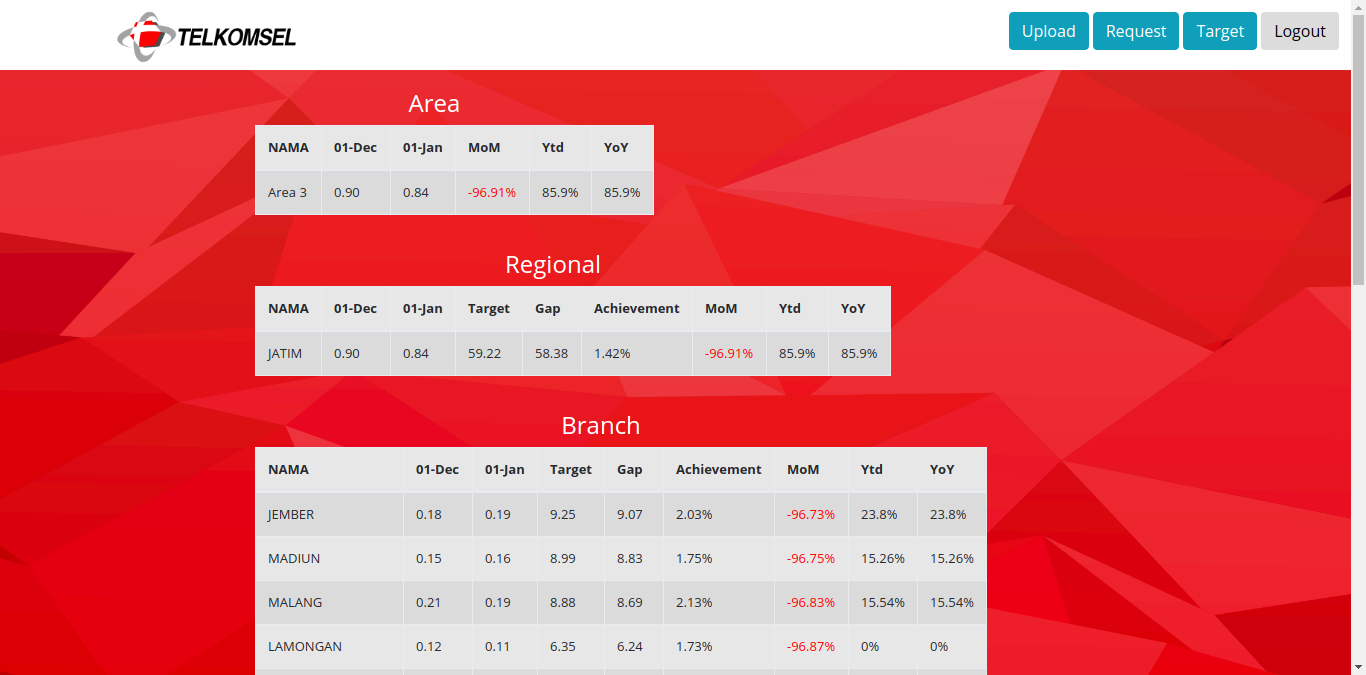
\includegraphics[width=10cm,height=5cm]{bab5/tampilanDetailPencapaian.png}}
	\caption{Halaman Detail Pencapaian \textit{Revenue}}
	\label{figure:pencapaianTPORT}
\end{figure}

\begin{figure}[h!]
	\centerline
	{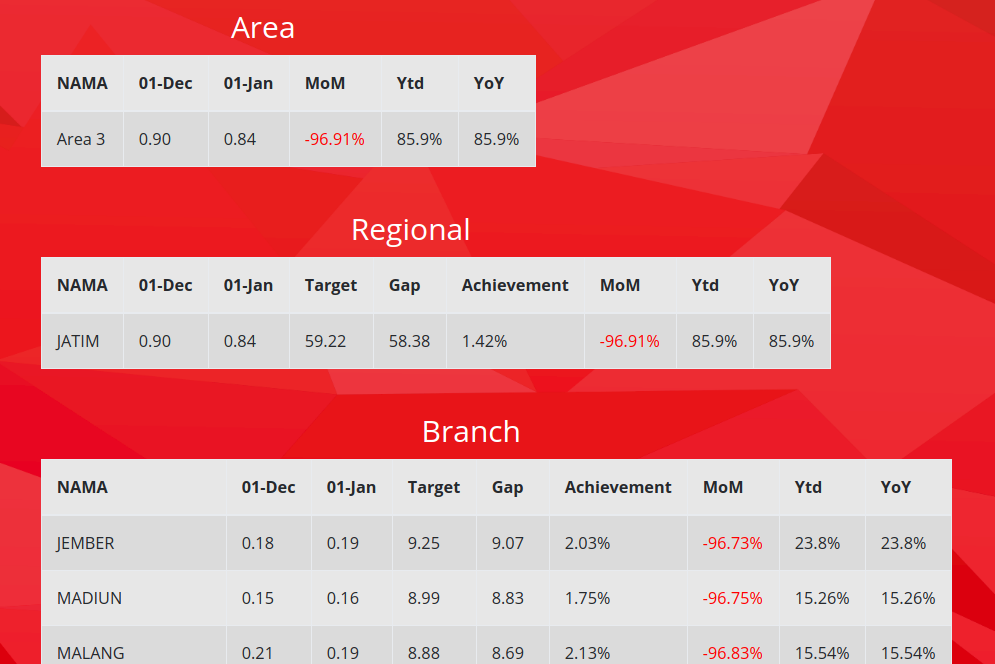
\includegraphics[width=9cm,height=6cm]{bab5/detailTampilanPencapaian.png}}
	\caption{Detail Halaman Pencapaian \textit{Revenue}}
	\label{figure:detailPencapaianTPORT}
\end{figure}

\lstinputlisting[language=PHP, firstline=1, lastline=24, firstnumber=1, caption=Potongan Kode Tampilan Target TPORT, label={lst:pencapaianTPORT}]{bab5/src/halamanDetail.php}
